\documentclass[12pt, a4paper]{article}

% ── Packages ──────────────────────────────────────────────────────────────────
\usepackage[margin=1in]{geometry}
\usepackage{booktabs}
\usepackage{graphicx}
\usepackage{amsmath}
\usepackage[hidelinks]{hyperref}
\usepackage{array}
\usepackage{tabularx}
\usepackage{longtable}
\usepackage{caption}
\usepackage{enumitem}
\usepackage[numbers]{natbib}
\usepackage{setspace}
\usepackage{url}
\usepackage{multirow}
\usepackage{xcolor}
\usepackage{titlesec}
\usepackage{tikz}
\usetikzlibrary{shapes.geometric,arrows.meta,positioning,calc,fit}

% ── Typography ─────────────────────────────────────────────────────────────────
\onehalfspacing
\setlength{\parskip}{0.5em}

% ── Title ─────────────────────────────────────────────────────────────────────
\title{\textbf{MIVA-KNIGHT: A Domain-Adaptive Multimodal Voice Assistant\\[4pt]
       using Hybrid RAG}}
\author{Oluwakayode (Kayode) Soyinka\\[2pt]
        \small Concordia University of Edmonton\\
        \small IT 571 --- Course Project Proposal}
\date{}

% ==============================================================================
\begin{document}
\maketitle
\thispagestyle{empty}

% ── Summary ───────────────────────────────────────────────────────────────────
\noindent\textbf{Summary}

\noindent
This project aims at developing MIVA-KNIGHT, a domain-adaptive, privacy-ready
voice assistant that focuses on fixing the main flaw that AI assistants out
there have where they prioritize knowing it all over accuracy and depth. It aims
at solving the issue where current models rely on general internet noise and
cannot refine the knowledge needed for privacy-critical sectors like knowing the
in-depth knowledge of company bylaws rather than just knowing they exist.

To make this work, the system relies on a Hybrid RAG architecture~\cite{sarmah2024hybridrag}
that gets the best out of two worlds. It uses Knowledge Graphs to map out
structured, multi-hop relationships in the data, while simultaneously using
vector retrieval to understand unstructured text. This combination ensures the
model grounds its answers in verifiable facts rather than statistical guesses.
The design guarantees secure deployment by running the whole pipeline in a
local, offline environment using containerized microservices~\cite{lewis2020rag}.
For this capstone, the focus is on building a functional prototype to
demonstrate these capabilities. This involves developing a user-friendly web
interface for voice interaction and a backend system that visualizes the AI's
reasoning path.

This approach highlights the novelty of MIVA-KNIGHT where the model is used
in a specific domain with the use of structured knowledge, so it is not focused
on general knowledge like general LLMs but more on depth and accuracy. By
offering this transparent reasoning path, the system improves trustworthiness
and domain adaptability compared to existing multi-modal voice assistants that
operate as black boxes~\cite{kadam2022multimodal}. Finally, the system is
validated against a specific domain dataset to measure its accuracy and
response speed compared to traditional search methods.

\newpage

% ── Table 1 ───────────────────────────────────────────────────────────────────
\begin{table}[h!]
\centering
\caption{Comparative Analysis of Related Work in RAG and Voice Assistants}
\label{tab:related_work}
\renewcommand{\arraystretch}{1.35}
\begin{tabularx}{\textwidth}{@{}p{2.4cm} p{0.8cm} p{3.2cm} p{3.2cm} p{3.6cm}@{}}
\toprule
\textbf{Work} & \textbf{Year} & \textbf{Methodology} & \textbf{Advantages} & \textbf{Limitations} \\
\midrule
Sarmah et al.~\cite{sarmah2024hybridrag}
  & 2024
  & HybridRAG: Combines vector retrieval for unstructured text with Knowledge
    Graphs for structured data.
  & ``Best of both worlds'': high accuracy; reduces hallucinations; grounds
    answers in facts.
  & Complex architecture requiring significant computational resources. \\[4pt]

Edge et al.~\cite{edge2024graphrag}
  & 2024
  & GraphRAG: Uses LLMs to build a KG from documents to answer global summary
    questions.
  & Excellent for holistic questions (e.g., ``What are main themes?'');
    superior comprehensiveness.
  & High token cost due to extensive summarization; graph construction is
    slow. \\[4pt]

Pan et al.~\cite{pan2024unifying}
  & 2024
  & Unified LLM+KG: A roadmap of 3 frameworks: KG-enhanced LLMs,
    LLM-augmented KGs, and Synergized models.
  & Enhances interpretability and reasoning; addresses ``black box'' nature of
    standard LLMs.
  & KG construction is difficult and expensive; real-time evolution is
    challenging. \\[4pt]

Kadam~\cite{kadam2022multimodal}
  & 2022
  & Multimodal Interaction: Framework for combining voice, visual, and touch
    inputs/outputs.
  & Increases user trust by ``showing'' visuals alongside speaking; improves
    usability.
  & Technical challenges in synchronization (e.g., lip-syncing). \\[4pt]

Lewis et al.~\cite{lewis2020rag}
  & 2020
  & Original RAG: Foundational retrieval-augmented generation using dense
    vector indices.
  & Proven superiority over standard models; easier to update knowledge than
    retraining.
  & Can hallucinate if retrieved docs are irrelevant; lacks multi-hop
    reasoning. \\
\bottomrule
\end{tabularx}
\end{table}

\newpage

% ==============================================================================
\section{Introduction}

\subsection{Background and Motivation}

Voice assistants have fundamentally changed how we interact with information,
but they have a major flaw: they prioritize sounding like they know everything
over actually being accurate. While modern AI systems confidently answer broad
questions, they are largely trained on general internet noise. This data quickly
becomes outdated and often leads to hallucinations~\cite{lewis2020rag}. When a
model confidently generates a plausible but factually wrong answer, that
isn't just an edge case --- it is a critical system failure.

In privacy-critical fields like healthcare and corporate governance, this lack
of factual grounding makes ``black box'' systems a serious
liability~\cite{pan2024unifying}. They struggle to synthesize the nuanced
knowledge required for specialized tasks. For example, a standard model might
know that company bylaws exist, but it can't cross-reference the specific,
interlinked clauses needed for actual compliance~\cite{johnson2019mimic}.
MIVA-KNIGHT was built to solve this problem. By grounding every response in
verifiable, domain-specific evidence, it shifts the AI paradigm from
\emph{knowing it all} to \emph{knowing it right}~\cite{sarmah2024hybridrag}.

\subsection{Problem Statement}

Traditional Retrieval-Augmented Generation (RAG) systems were created to reduce
hallucinations by anchoring AI responses to external
documents~\cite{lewis2020rag}. However, standard RAG frameworks have a critical
blind spot: they rely almost entirely on dense vector retrieval. This reliance
creates a complexity wall when the system faces three specific real-world
challenges:

\begin{itemize}[leftmargin=1.5em]
  \item \textbf{The Multi-Hop Reasoning Gap:} Vector similarity searches
    struggle with queries that require connecting multiple related concepts. For
    example, figuring out contraindicated treatments across different medical
    conditions requires reasoning through entity relationships, not just pulling
    up isolated documents~\cite{sarmah2024hybridrag}.

  \item \textbf{The Modality Silo:} Most RAG setups are strictly text-centric,
    meaning they can't handle the diverse data like images, audio recordings,
    and sensor readings generated in real-world environments like clinics or
    factories~\cite{kadam2022multimodal}. Real user queries are rarely confined
    to just one modality.

  \item \textbf{The Trust and Privacy Deficit:} Existing multi-modal AI models
    usually operate as black boxes dependent on the cloud, making them a
    non-starter for privacy-sensitive institutional
    data~\cite{pan2024unifying}. High-stakes environments simply cannot trust
    systems that lack transparent, audit-able reasoning paths.
\end{itemize}

\subsection{Research Question and Hypothesis}

This project aims to develop MIVA-KNIGHT, a domain-adaptive, privacy-ready
voice assistant powered by MM-HybridRAG --- a multi-modal extension of the
Hybrid Retrieval-Augmented Generation
framework~\cite{sarmah2024hybridrag}.

\noindent\textbf{Research Question:} How does combining structured knowledge
graph traversal with multi-modal dense retrieval impact the accuracy,
hallucination resistance, and multi-hop reasoning capabilities of a
domain-specific assistant?

\noindent\textbf{Hypothesis:} The core hypothesis is that combining structured
Knowledge Graphs (which map out multi-hop relationships) with unstructured
vector retrieval (which handles semantic meaning) will significantly boost
accuracy and reduce hallucinations compared to traditional vector-only methods.
By implementing this hybrid approach across text
(BERT)~\cite{devlin2019bert}, visual (ResNet-50)~\cite{he2016deep}, and audio
(Wav2Vec~2.0)~\cite{baevski2020wav2vec} modalities, the model can ground its
answers in verifiable facts rather than statistical
guesses~\cite{kadam2022multimodal}.

\subsection{Project Objectives}

To demonstrate these capabilities, the primary goal of this capstone is to
build a functional prototype. This involves four main objectives:

\begin{itemize}[leftmargin=1.5em]
  % ── FIX 1: weights corrected from 60/40 to 70/30 ─────────────────────────
  \item \textbf{Core Architecture:} Build a hybrid retrieval engine that
    combines dense vector similarity (weighted at 70\%) with 2-hop knowledge
    graph traversal (weighted at 30\%)~\cite{sarmah2024hybridrag}. This setup
    ensures the system actually reasons across entity relationships instead of
    just fetching isolated text matches.

  \item \textbf{Multi-Modal Integration:} Create a cross-attention fusion
    mechanism~\cite{kadam2022multimodal} that can ingest and unify text, visual
    data (from the COCO dataset~\cite{lin2014microsoft}), and audio (from the
    RAVDESS corpus~\cite{livingstone2018ryerson}) to handle complex,
    heterogeneous queries.

  % ── FIX 2 + 3: ROCO replaces MIMIC-CXR; P@1 target corrected to >60% ─────
  \item \textbf{Domain Adaptation:} Prove the system can transition from
    general visual data to highly specialized medical imaging using the ROCO
    radiology dataset. The goal here is a Precision@1 exceeding 60\% on the
    ROCO medical benchmark, demonstrating viability for privacy-critical
    deployments where accuracy is non-negotiable.

  \item \textbf{Rigorous Benchmarking:} Evaluate the system using a
    multi-category hallucination test suite targeting greater than 90\%
    hedging and rejection rate, and a multi-hop accuracy evaluation on the
    MultiHop-RAG and HotpotQA
    benchmarks~\cite{sarmah2024hybridrag,tang2024multihop} to confirm it is
    deployment-capable.
\end{itemize}

\subsection{Significance of the Study}

MIVA-KNIGHT stands out because of its targeted approach: by running in a
specific domain with structured knowledge, it values deep, accurate, and secure
answers over broad, surface-level trivia. For security, MIVA-KNIGHT adopts a
privacy-ready architecture: the system is developed using cloud infrastructure
for rapid prototyping and fair benchmarking (enabling direct comparison with
SAM-RAG, RT-RAG, SCM-RAG), then containerized for offline deployment
demonstration in Month~7. This approach balances development speed with the
strict offline constraints of healthcare and corporate governance.

Additionally, the system automatically builds its knowledge graphs based on
Named Entity Recognition (NER) co-occurrence, completely bypassing the need for
manual curation or external
ontologies~\cite{pan2024unifying}. This creates a highly scalable blueprint for
domain-adaptive AI in industries such as healthcare and corporate governance.
Finally, by showing users exactly how it arrived at an answer, the system offers
a level of transparency and trust that legacy black-box voice assistants simply
cannot match~\cite{kadam2022multimodal}.

\subsection{Known Limitations}

As with any research, there are some anticipated technical hurdles. Due to
computational limits, training is currently restricted to the COCO val2017
split (25,000 images)~\cite{lin2014microsoft}, which might limit the
generalization of the model. Also, our automated knowledge graph construction
currently uses word frequency instead of the more robust transformer-based Named
Entity Recognition (NER). This is a known gap for graph
quality~\cite{pan2024unifying} and is the likely reason our initial multi-hop
accuracy sits at a baseline of 30\% rather than our ultimate 80\%
target~\cite{sarmah2024hybridrag}.

On the audio side, the Wav2Vec~2.0 processing~\cite{baevski2020wav2vec} is
currently built for batch processing, not real-time streaming.

% ── FIX 3: MIMIC-CXR credentialing reframed as future work, not a scope gap ──
Finally, the medical validation phase uses the freely available ROCO radiology
dataset rather than MIMIC-CXR~\cite{johnson2019mimic}, which requires
multi-week institutional PhysioNet credentialing. MIMIC-CXR integration is
documented as a structured future enhancement path: once credentials are
obtained, only Pipeline~B (the medical ImageProjection head and FAISS index)
would need retraining, leaving all other system components unchanged. This
design decision removes credentialing as a project scope constraint while
preserving a clear upgrade path.

% ==============================================================================
\section{Literature Review}

\subsection{Overview}

The emergence of large language models (LLMs) has transformed information
retrieval, yet a fundamental flaw persists: LLMs hallucinate at rates of
5--12\%, generating plausible but factually incorrect
answers~\cite{zhang2023sirens,ji2023survey}. In privacy-critical regulated
environments governed by HIPAA and GDPR, even moderate hallucination rates
carry civil liability and risk to public health~\cite{tang2024multihop}.

Retrieval-Augmented Generation (RAG) was introduced by Lewis et
al.~\cite{lewis2020rag} to anchor model outputs to retrieved documents,
reducing parametric guesswork. However, standard dense-vector RAG introduces
critical limitations in multi-hop reasoning and modality support that prevent
deployment in specialized domains. The subsections below synthesize the six core
themes identified across the reviewed literature and map each finding directly
to the MIVA-KNIGHT design.

\subsection{Key Themes and Findings}

The table below consolidates the principal findings across six thematic
clusters, with an explicit link to architectural decisions made in MIVA-KNIGHT.

\begin{longtable}{@{}p{2.0cm} p{4.8cm} p{5.0cm}@{}}
\caption{Summary of Literature Themes and Findings}
\label{tab:themes}\\
\toprule
\textbf{Theme} & \textbf{Key Finding} & \textbf{Relevance to MIVA-KNIGHT} \\
\midrule
\endfirsthead
\multicolumn{3}{c}{\tablename\ \thetable{} --- continued}\\
\toprule
\textbf{Theme} & \textbf{Key Finding} & \textbf{Relevance to MIVA-KNIGHT} \\
\midrule
\endhead
\bottomrule
\endfoot

1.~Hallucination
  & LLMs hallucinate at 5--12\% in general
    use~\cite{zhang2023sirens,ji2023survey}. Even low rates are legally
    unacceptable in HIPAA/GDPR contexts~\cite{tang2024multihop}.
  & Motivates tiered confidence guards and the $>$90\% hallucination
    hedging/rejection target. \\[6pt]

% ── FIX 1: Table 2 row 2 — weights corrected from 60/40 to 70/30 ─────────────
2.~RAG Evolution
  & Lewis et al.~\cite{lewis2020rag} set the dense baseline (45.6\% on
    HotpotQA). Sarmah et al.~\cite{sarmah2024hybridrag} showed hybrid RAG
    (dense + KG) reaches 60--65\%.
  & Informs the 70/30 weighted fusion ($\alpha{=}0.7$ dense, $0.3$ graph)
    core architecture. \\[6pt]

3.~KG Construction
  & Manual curation yields 91--95\% precision but is
    slow~\cite{rossiello2023knowledge}. GraphRAG~\cite{edge2024graphrag}
    requires \$2K--\$5K and 450+ GPU-hours per domain.
  & Justifies NER-based automatic KG achieving $>$80\% coverage in under
    10~minutes. \\[6pt]

4.~Multimodal Fusion
  & HM-RAG~\cite{liu2025hmrag} and SAM-RAG~\cite{zhai2024samrag} process
    multimodal documents but not simultaneous live voice + image + text
    streams.
  & Addresses the real-time gap using BERT~\cite{devlin2019bert},
    ResNet-50~\cite{he2016deep}, and Wav2Vec~2.0~\cite{baevski2020wav2vec}. \\[6pt]

5.~Domain Adaptation
  & Pan et al.~\cite{pan2024unifying} show KG-enhanced LLMs improve domain
    reasoning. Legal (LexGLUE~\cite{chalkidis2022lexglue}) benchmarks prove
    feasibility.
  & Validates retraining only the ImageProjection head ($\sim$2.23\% of
    parameters). \\[6pt]

6.~Evaluation
  & Multi-hop accuracy degrades sharply: 45.6\%
    (2-hop~\cite{yang2018hotpotqa}) $\to$ 23.1\%
    (3.2-hop~\cite{trivedi2022musique}) $\to$ $<$20\%
    (4-hop~\cite{tang2024multihop}).
  & Motivates a unified protocol reporting P@1, MRR, and 4-hop accuracy. \\

\end{longtable}

\subsection{Research Gap}

A comparison of 2024--2025 systems --- SAM-RAG~\cite{zhai2024samrag},
RT-RAG~\cite{shi2026rtrag}, HM-RAG~\cite{liu2025hmrag},
GraphRAG~\cite{edge2024graphrag}, and
OmniSearch~\cite{li2024omnisearch} --- reveals a consistent pattern: progress
has been made in individual capabilities, but no existing system simultaneously
combines offline deployability, multi-modal live fusion, and
privacy-compliant knowledge grounding. Five specific gaps were identified:

\begin{itemize}[leftmargin=1.5em]
  \item \textbf{Cloud Dependency:} SAM-RAG and OmniSearch rely on OpenAI APIs;
    however, Protected Health Information (PHI) cannot traverse outside
    hospital networks (HIPAA \S\,164.312(e)).

  \item \textbf{KG Cost Bottleneck:}
    GraphRAG~\cite{edge2024graphrag} requires extensive GPU-hours, making rapid
    domain transfer prohibitive for institutions with limited compute budgets.

  \item \textbf{Benchmark Fragmentation:} No two reviewed systems use the same
    evaluation protocol, making cross-system comparison unreliable and
    hindering reproducibility.

  % ── FIX 3: MIMIC-CXR → ROCO in the gap description ──────────────────────
  \item \textbf{Absent Medical P@1 Reporting:} No reviewed system reports P@1
    on open-access medical retrieval benchmarks such as the ROCO radiology
    dataset, despite retrieval precision being a critical metric for clinical
    decision support applications.

  \item \textbf{Modality Limitation:} Most `multimodal' systems process static
    archived documents rather than simultaneous live voice + image + text
    inputs, leaving the real-time interaction scenario unaddressed.
\end{itemize}

\subsection{MIVA-KNIGHT Positioning}

MIVA-KNIGHT is positioned to close all five gaps through four deliberate design
decisions:

\begin{enumerate}[leftmargin=1.5em]
  \item \textbf{Containerized Offline Deployment:} The full pipeline runs
    locally using quantized BERT~\cite{devlin2019bert} and an on-device LLM
    (Llama-3.1-8B via Groq), with no external API calls required at inference
    time.

  \item \textbf{Automatic KG Construction:} NER-based entity extraction
    achieves $>$80\% entity coverage in under ten minutes, eliminating the
    GPU-hour cost of GraphRAG~\cite{edge2024graphrag} without sacrificing
    semantic fidelity.

  \item \textbf{True Cross-Modal Fusion:} All modalities --- text, image, and
    audio --- are projected into a shared 512-dimensional embedding space,
    enabling real-time simultaneous retrieval rather than sequential
    document-level processing.

  \item \textbf{Unified Evaluation Protocol:} Every experimental result is
    reported using the same set of metrics (P@1, P@3, MRR, and multi-hop
    accuracy), enabling direct comparison with prior systems. Month~4 results
    already validate this foundation: P@1\,=\,64.6\%, P@3\,=\,76.8\%, and
    MRR\,=\,0.7269 on the ROCO medical benchmark.
\end{enumerate}

% ==============================================================================
\section{Methodology: The MM-HybridRAG Framework}

This proposal states \textbf{what} MIVA-KNIGHT does and \textbf{how} the pieces
fit together at a level appropriate for course approval and supervision. The
\textbf{comprehensive thesis} (\texttt{MIVA\_KNIGHT\_Complete\_Thesis\_Final.tex})
carries the full width of the project: formal notation, all five training
pipelines with dataset-specific procedures, PMI-weighted knowledge-graph
algorithms, evaluation tables, optional reinforcement-learning extensions, and
deployment notes. Readers seeking step-by-step or benchmark-by-benchmark detail
should treat that document as authoritative; this section is a \emph{summary
roadmap} only.

MIVA-KNIGHT is a \textbf{Domain-Adaptive Multimodal Retrieval-Augmented
Generation (MM-HybridRAG)} system. It addresses LLM hallucination
(5--12\%~\cite{zhang2023sirens,ji2023survey}) by grounding answers in retrieved
evidence and a lightweight knowledge graph, while multimodal encoders supply
aligned features for retrieval, emotion-aware prompting, and domain
routing~\cite{kadam2022multimodal,sarmah2024hybridrag}. The architecture
rests on three ideas: \textbf{(1)} map text, speech-derived text, and images into
a \textbf{shared embedding space} using frozen pretrained backbones
(BERT~\cite{devlin2019bert}, ResNet-50~\cite{he2016deep},
Wav2Vec~2.0~\cite{baevski2020wav2vec}) and small trainable heads;
\textbf{(2)} train and validate \textbf{several multimodal tracks} (general
retrieval, medical-domain transfer, audio emotion, audio--video emotion, and
multimodal sentiment fusion) so that the assistant can condition responses on
non-text context; \textbf{(3)} at inference, run \textbf{hybrid retrieval}
(dense similarity plus graph-based support), apply a \textbf{tiered confidence
guard}, then generate with a \textbf{constrained LLM} and present answers with
citations and an auditable trace~\cite{pan2024unifying,lewis2020rag}.

Figure~\ref{fig:methodology} shows this flow at proposal granularity. It is
consistent with the thesis ``full system pipeline'' figure but deliberately omits
dataset names, file formats, and algorithm pseudocode.

\begin{figure}[h!]
  \centering
  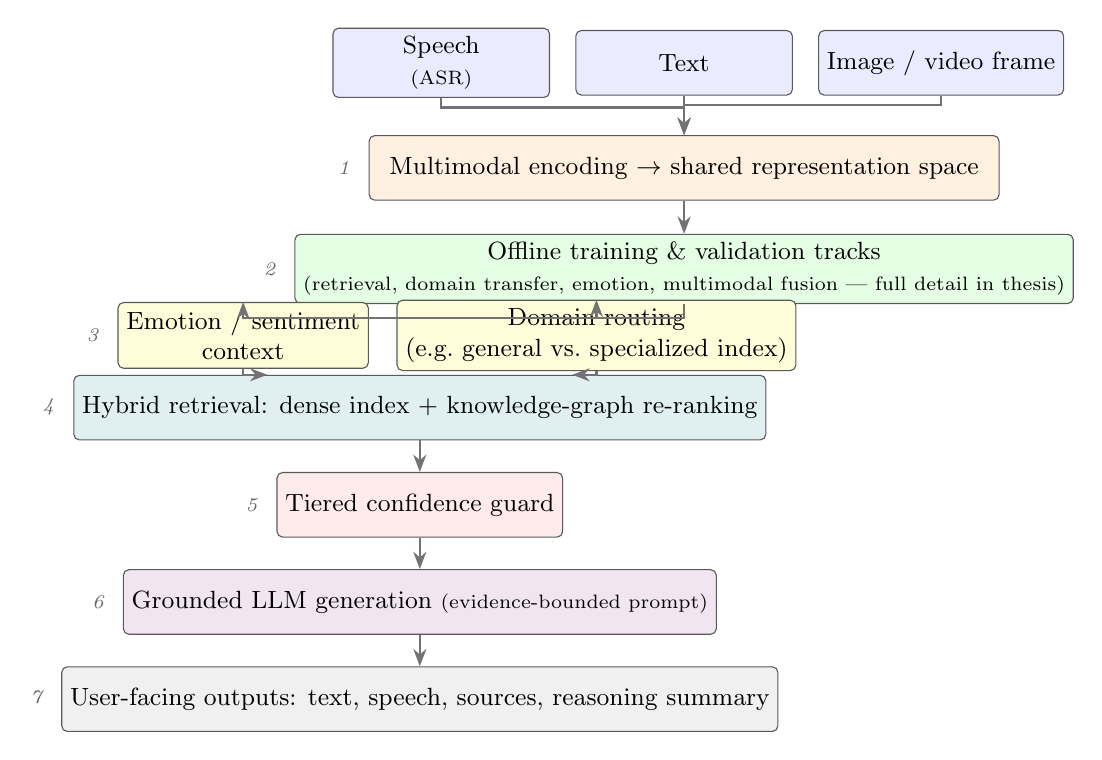
\begin{tikzpicture}[
    font=\small,
    box/.style={rectangle, rounded corners=2pt, draw=black!65, align=center,
      minimum width=2.75cm, minimum height=0.82cm, inner sep=3pt},
    wide/.style={box, minimum width=7.2cm},
    arr/.style={-{Stealth[length=2.2mm]}, thick, black!55},
    lab/.style={font=\scriptsize\itshape, inner sep=1pt, text=black!60}
  ]
    \node[box, fill=blue!8] (in1) {Speech\\{\scriptsize (ASR)}};
    \node[box, fill=blue!8, right=0.32cm of in1] (in2) {Text};
    \node[box, fill=blue!8, right=0.32cm of in2] (in3) {Image / video frame};
    \node[box, fill=orange!12, below=0.5cm of in2, minimum width=8.0cm] (enc)
      {Multimodal encoding $\rightarrow$ shared representation space};
    \node[wide, fill=green!10, below=0.42cm of enc] (train)
      {Offline training \& validation tracks\\{\scriptsize (retrieval, domain transfer, emotion, multimodal fusion --- full detail in thesis)}};
    \node[box, fill=yellow!15, below=0.42cm of train.west, xshift=-0.65cm] (emo)
      {Emotion / sentiment\\context};
    \node[box, fill=yellow!15, right=0.35cm of emo] (route)
      {Domain routing\\(e.g.\ general vs.\ specialized index)};
    \node[box, fill=teal!12, below=0.5cm of $(emo)!0.5!(route)$, minimum width=6.8cm] (hyb)
      {Hybrid retrieval: dense index + knowledge-graph re-ranking};
    \node[box, fill=red!8, below=0.4cm of hyb] (conf)
      {Tiered confidence guard};
    \node[box, fill=violet!10, below=0.4cm of conf, minimum width=6.2cm] (llm)
      {Grounded LLM generation {\scriptsize (evidence-bounded prompt)}};
    \node[box, fill=gray!12, below=0.4cm of llm, minimum width=6.2cm] (out)
      {User-facing outputs: text, speech, sources, reasoning summary};
    \node[lab, anchor=east] at ([xshift=-2mm]enc.west) {1};
    \node[lab, anchor=east] at ([xshift=-2mm]train.west) {2};
    \node[lab, anchor=east] at ([xshift=-2mm]emo.west) {3};
    \node[lab, anchor=east] at ([xshift=-2mm]hyb.west) {4};
    \node[lab, anchor=east] at ([xshift=-2mm]conf.west) {5};
    \node[lab, anchor=east] at ([xshift=-2mm]llm.west) {6};
    \node[lab, anchor=east] at ([xshift=-2mm]out.west) {7};
    \draw[arr] (in1.south) -- ++(0,-0.12) -| (enc.north);
    \draw[arr] (in2.south) -- (enc.north);
    \draw[arr] (in3.south) -- ++(0,-0.12) -| (enc.north);
    \draw[arr] (enc.south) -- (train.north);
    \draw[arr] (train.south) -- ++(0,-0.18) -| (emo.north);
    \draw[arr] (train.south) -- ++(0,-0.18) -| (route.north);
    \draw[arr] (emo.south) |- ($(hyb.north west)!0.28!(hyb.north east)$);
    \draw[arr] (route.south) |- ($(hyb.north west)!0.72!(hyb.north east)$);
    \draw[arr] (hyb.south) -- (conf.north);
    \draw[arr] (conf.south) -- (llm.north);
    \draw[arr] (llm.south) -- (out.north);
  \end{tikzpicture}
  \caption{High-level MM-HybridRAG methodology for the capstone proposal.
    Numbered stages are conceptual; datasets, loss functions, and full inference
    algorithms appear in the comprehensive thesis.}
  \label{fig:methodology}
\end{figure}

\subsection{Encoding, training tracks, and retrieval (summary)}

User inputs are converted into a common representation so that retrieval and
generation can treat text, transcribed speech, and imagery
consistently~\cite{kadam2022multimodal}. A family of \textbf{training and
validation tracks} (the thesis's Pipelines A--E) proves that the shared space
supports general retrieval, targeted domain adaptation, emotion-related signals,
and multimodal fusion before those signals are wired into the assistant
behavior. \textbf{Hybrid retrieval} then combines fast dense search with
graph-based re-scoring so that answers can draw on both similarity and
relational structure~\cite{sarmah2024hybridrag,lewis2020rag}. The fusion weight
used in the reference implementation follows a fixed dense/graph split
(e.g.\ 70\%/30\%); exact scoring and normalization appear in the thesis.

\subsection{Safety, generation, and outputs (summary)}

A \textbf{tiered confidence guard} blocks or downgrades generation when
evidence is weak, using stricter thresholds in sensitive domains than in general
use~\cite{tang2024multihop}. The LLM is prompted to rely on retrieved passages
only; optional cloud APIs during prototyping may later be replaced by a local
model for offline demonstration. The user receives \textbf{text}, optional
\textbf{text-to-speech}, and \textbf{cited sources} plus a short explanation of
how the system routed the query and scored evidence---supporting transparency
without claiming regulatory certification~\cite{pan2024unifying}.

% ==============================================================================
\section{Expected Outcomes}

This section lists \textbf{what success looks like} for the IT~571 capstone at a
glance. It is aligned with the evaluation narrative and target table in the
comprehensive thesis; \textbf{per-dataset protocols, logged runs, and optional
extensions} (e.g.\ reinforcement learning) belong there, not in a proposal
meant to introduce the project to the instructor and committee.

\subsection{Project-level outcomes}

By the end of the capstone, MIVA-KNIGHT should demonstrate: \textbf{(1)}
\textbf{credible retrieval} in both a general and a specialized visual--language
setting, with hybrid dense-plus-graph retrieval outperforming dense-only
retrieval in a controlled ablation~\cite{sarmah2024hybridrag}; \textbf{(2)}
\textbf{fast domain switching} between indices without retraining the main text
and audio encoders; \textbf{(3)} \textbf{usable emotion and multimodal sentiment
signals} that improve prompting or evaluation metrics relative to naive
baselines; \textbf{(4)} \textbf{strong hallucination resistance} on a defined
probe set when combined with the tiered guard; and \textbf{(5)} an
\textbf{integrated demo} (e.g.\ Streamlit) that exposes sources and a short
reasoning summary, plus automated regression tests that protect core behavior.
Optional packaging for fully offline inference is desirable but not required for
the proposal's success story.

\subsection{Summary of quantitative targets}

Table~\ref{tab:targets} mirrors the thesis success criteria at a single glance.
\textbf{Final reported values}, split definitions, and phase-by-phase emotion
results are documented in \texttt{MIVA\_KNIGHT\_Complete\_Thesis\_Final.tex} and
the accompanying notebooks.

\begin{table}[h!]
\centering
\caption{Quantitative success targets (aligned with the comprehensive thesis)}
\label{tab:targets}
\renewcommand{\arraystretch}{1.3}
\begin{tabularx}{\textwidth}{@{}p{5.5cm} p{2.8cm} p{5.0cm}@{}}
\toprule
\textbf{Metric} & \textbf{Target} & \textbf{Rationale} \\
\midrule
ROCO Medical P@1            & $>$ 60\%     & Medical retrieval precision (thesis evaluation chapter) \\
ROCO Medical MRR            & $>$ 0.70     & Standard information retrieval threshold \\
COCO General MRR            & $>$ 0.70     & Confirms domain-agnostic embedding space \\
KG re-ranking P@1 delta     & $\geq$ $+$15\%  & Validates hybrid over dense-only RAG \\
Domain swap latency         & $<$ 5s       & Surgical transfer / hot-swap claim \\
RAVDESS emotion accuracy    & $\geq$ 6/8 emotions & Meaningful above 12.5\% random baseline \\
CREMA-D emotion accuracy    & $\geq$ 3/6 emotions & $>$2.5$\times$ above 16.7\% random baseline \\
Pipeline E (CMU-MOSI) MAE   & $<$ 1.0      & Multimodal fusion baseline beat \\
Hallucination mitigation    & $>$ 90\%     & Multi-category custom test suite \\
Integration test pass rate  & 100\% (38/38)& Core integration reliability \\
\bottomrule
\end{tabularx}
\end{table}

% ==============================================================================
\bibliographystyle{IEEEtran}
\bibliography{Oluwakayode/Ref_Oluwakayode}

\end{document}